Quoting
\href{https://mastodon.macstories.net/}{@viticci@mastodon.macstories.net}:
\url{https://mastodon.macstories.net/@viticci/111818291056052593}
\#retoot

\begin{figure}
\centering
\pandocbounded{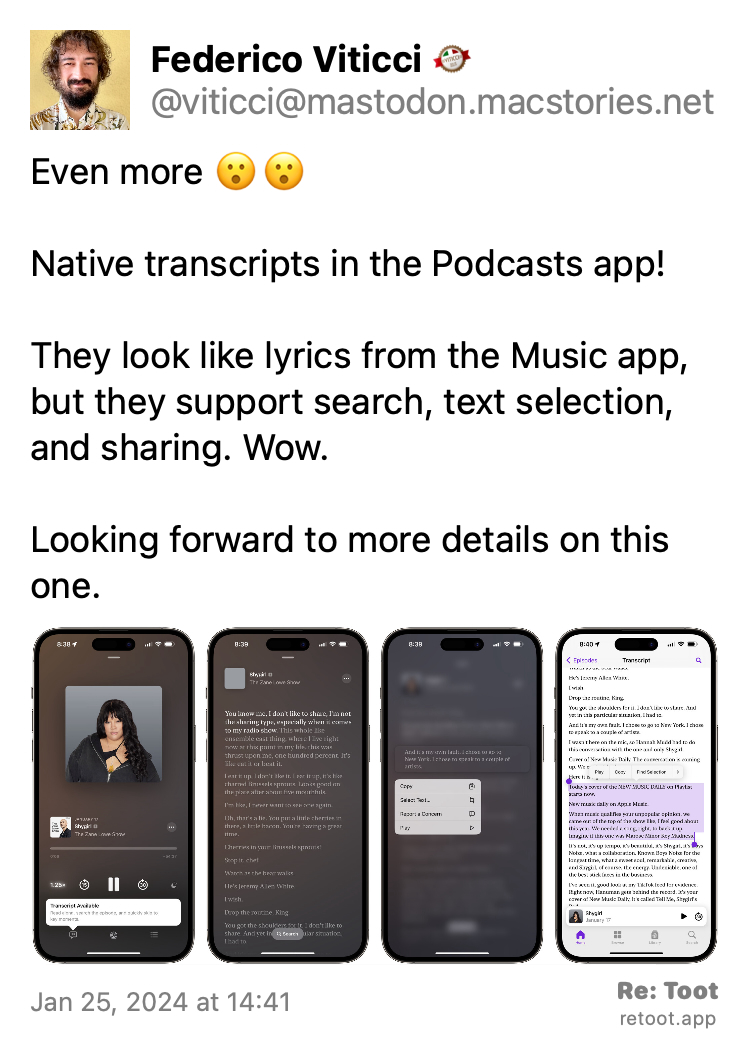
\includegraphics[keepaspectratio]{\%7B\%7Bsite.url\%7D\%7D/img/transcripts-A.jpg}}
\caption{Post by Federico Viticci. ``Even more 😮😮 Native transcripts
in the Podcasts app! They look like lyrics from the Music app, but they
support search, text selection, and sharing. Wow. Looking forward to
more details on this one.'' The post contains an image with no
description. Posted on Jan 25, 2024 at 14:41}
\end{figure}

\begin{quote}
\emph{Post by Federico Viticci. ``Even more 😮😮 Native transcripts in
the Podcasts app! They look like lyrics from the Music app, but they
support search, text selection, and sharing. Wow. Looking forward to
more details on this one.'' The post contains an image with no
description. Posted on Jan 25, 2024 at 14:41}
\end{quote}

Quoting
\href{https://zeppelin.flights/@jsnell/}{@jsnell@zeppelin.flights}:
\url{https://zeppelin.flights/@jsnell/111818570023689131} \#retoot

\begin{figure}
\centering
\pandocbounded{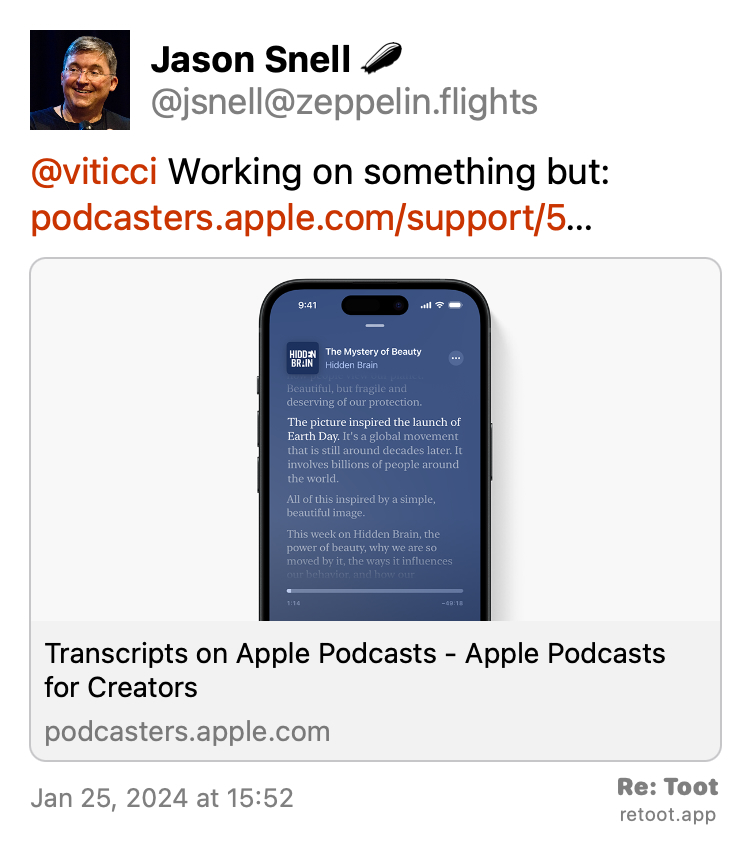
\includegraphics[keepaspectratio]{\%7B\%7Bsite.url\%7D\%7D/img/transcripts-B.jpg}}
\caption{Post by Jason Snell. ``@viticci Working on something but:
podcasters.apple.com/support/5\ldots{}'' Posted on Jan 25, 2024 at
15:52}
\end{figure}

\begin{quote}
\emph{Post by Jason Snell. ``@viticci Working on something but:
podcasters.apple.com/support/5\ldots{}'' Posted on Jan 25, 2024 at
15:52}
\end{quote}

Link that Jason was linking to:
\url{https://web.archive.org/web/20240125222508/https://podcasters.apple.com/support/5316-transcripts-on-apple-podcasts}

Quoting
\href{https://mastodon.social/@samburkhard/}{@samburkhard@mastodon.social}:
\url{https://mastodon.social/@samburkhard/111818919630257996} \#retoot

\begin{figure}
\centering
\pandocbounded{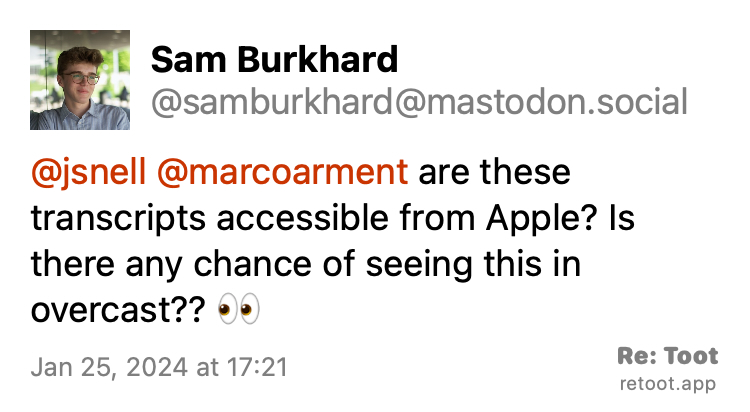
\includegraphics[keepaspectratio]{\%7B\%7Bsite.url\%7D\%7D/img/transcripts-C.jpg}}
\caption{Post by Sam Burkhard. ``@jsnell @marcoarment are these
transcripts accessible from Apple? Is there any chance of seeing this in
overcast?? 👀'' Posted on Jan 25, 2024 at 17:21}
\end{figure}

\begin{quote}
\emph{Post by Sam Burkhard. ``@jsnell @marcoarment are these transcripts
accessible from Apple? Is there any chance of seeing this in overcast??
👀'' Posted on Jan 25, 2024 at 17:21}
\end{quote}

Now for my reaction to all this! At present, I don't have a way to push
my own transcript using \href{https://www.acast.com}{Acast}. Presently I
am listening to podcasts using \href{https://overcast.fm}{Overcast}
instead of Apple's stock podcast app. Why use Overcast? It is easier to
keep podcast listening in sync between my tablet, phone, laptop, and
smartwatch.

Do I listen to podcasts from my smartwatch alone using a Bluetooth
headset connected to the smartwatch? Yes, I do. Walking the chihuahua in
the park is a good example of that. Using the treadmill at home is also
a good example. The stock Apple podcast app for my watch was just too
clumsy and cumbersome to use while Overwatch does what I want it to do
with far less hassle.

Are they using a Whisper-like LLM to do this transcription work? That's
the big unknown to this. Whisper is not perfect. It also might have
problems listening to \href{https://69admins.com}{69 Admins} to be able
to come up with \emph{good} transcript results.
